\documentclass[11pt,a4paper]{article}

% ---------------------------------------------------------------------------
% Exact overlap partitions and gateway scaling in Kauffman RAF networks.
%
% Author metadata: set the three macros below before submission.
% Build: see BUILD.md (pdflatex -> bibtex -> pdflatex -> pdflatex).
% ---------------------------------------------------------------------------
\newcommand{\PaperAuthor}{Anonymous manuscript}
\newcommand{\PaperAffiliation}{}
\newcommand{\PaperDate}{September 7, 2026}

\usepackage[T1]{fontenc}
\usepackage[utf8]{inputenc}
\usepackage{lmodern}
\usepackage{microtype}
\usepackage[a4paper,margin=1.05in]{geometry}
\usepackage{amsmath,amssymb,amsthm}
\usepackage{booktabs}
\usepackage{array}
\usepackage{enumitem}
\usepackage{xcolor}
\usepackage{graphicx}
\usepackage{tikz}
\usetikzlibrary{arrows.meta,positioning,calc}
\usepackage{url}
\usepackage[colorlinks=true,linkcolor=blue!55!black,citecolor=blue!55!black,urlcolor=blue!55!black]{hyperref}

\setlist{itemsep=2pt,topsep=3pt}
\setlength{\emergencystretch}{1.5em}

\theoremstyle{plain}
\newtheorem{theorem}{Theorem}[section]
\newtheorem{proposition}[theorem]{Proposition}
\newtheorem{lemma}[theorem]{Lemma}
\newtheorem{corollary}[theorem]{Corollary}
\theoremstyle{definition}
\newtheorem{definition}[theorem]{Definition}
\newtheorem{example}[theorem]{Example}
\newtheorem{conjecture}[theorem]{Conjecture}
\theoremstyle{remark}
\newtheorem{remark}[theorem]{Remark}
\newtheorem{question}[theorem]{Question}

% Lean identifiers: typewriter, with a discretionary break after every underscore
% and after every lower-to-upper camel-case boundary is not attempted; underscores
% occur in every long identifier used below.
\newcommand{\lean}[1]{\begingroup\def\_{\char`\_\allowbreak}\texttt{#1}\endgroup}
\newcommand{\RAF}{\mathrm{RAF}}
% Lean declaration names attached to a statement, on their own ragged line.
\newcommand{\leanrefs}[1]{\par\nopagebreak{\small\raggedright\textup{Lean: #1.}\par}}
\renewcommand{\Pr}{\operatorname{Pr}}
\newcommand{\cX}{\mathcal{X}}
\newcommand{\cJ}{\mathcal{J}}
\newcommand{\cK}{\mathcal{K}}
\newcommand{\cR}{\mathcal{R}}
\newcommand{\cF}{\mathcal{F}}
\newcommand{\cA}{\mathcal{A}}
\newcommand{\cC}{\mathcal{C}}
\newcommand{\cS}{\mathcal{S}}
\newcommand{\cT}{\mathcal{T}}
\newcommand{\cU}{\mathcal{U}}
\newcommand{\cW}{\mathcal{W}}
\newcommand{\cG}{\mathcal{G}}
\newcommand{\cE}{\mathcal{E}}
\newcommand{\cN}{\mathcal{N}}
\newcommand{\cV}{\mathcal{V}}
\newcommand{\cL}{\mathcal{L}}
\newcommand{\cB}{\mathcal{B}}
\newcommand{\cM}{\mathcal{M}}
\newcommand{\cO}{\mathcal{O}}
\newcommand{\cP}{\mathcal{P}}
\newcommand{\cQ}{\mathcal{Q}}
\newcommand{\lhs}{\operatorname{lhs}}
\newcommand{\rhs}{\operatorname{rhs}}
\newcommand{\cl}{\operatorname{cl}}
\newcommand{\core}{\operatorname{core}}
\newcommand{\seed}{\operatorname{Seed}}
\newcommand{\Nat}{\mathbb{N}}
\newcommand{\Real}{\mathbb{R}}
\newcommand{\Int}{\mathbb{Z}}
\newcommand{\Fin}{\mathbb{F}}
\newcommand{\pow}[1]{2^{#1}}
\newcommand{\ee}{\mathrm{e}}
\newcommand{\word}[1]{\mathtt{#1}}

\title{Exact Overlap Partitions and Gateway Scaling\\ in Kauffman RAF Networks}
\author{\PaperAuthor\\ \PaperAffiliation}
\date{\PaperDate}

\begin{document}
\maketitle

\begin{abstract}
We study the probability that a reflexively autocatalytic and food-generated (RAF) set exists in Kauffman's binary-polymer model with random catalysis, in the exact reaction convention of the public code accompanying the recent finite-core theory of RAF emergence of Varanasi and Korenaga. That theory assigns activation probabilities to minimal catalytic cores and, for tractability, treats the cores as non-overlapping. We remove the approximation. For any finite catalogue of candidate cores we prove an exact two-level inclusion--exclusion formula for the probability that at least one core is activated, valid both for independent Bernoulli catalysis and for a uniformly random set of exactly $Q$ catalysis assignments, and we prove that for the exhaustive catalogue of food-generated reaction supports the formula computes precisely the probability of the RAF event. The sufficient statistic is not a matrix of pairwise core overlaps: it is, for each reaction channel, the family of cardinalities of all unions of the eligible-catalyst sets of the selected cores. A four-molecule example shows that pairwise data cannot determine the answer. The independent-core formula of the finite-core theory is recovered exactly, and only, under the hypothesis of coordinate-disjoint cores. We then show that the fixed food set imposes a finite gateway. For every maximal polymer length $n\ge 4$ the repository convention has exactly $34$ reaction channels usable from food, and every RAF contains a catalysed one. Consequently, if $f_n$ is the expected number of channels catalysed per molecule, then $\Pr(\RAF_n)\le 272 f_n/n$ for $n\ge3$; $\Pr(\RAF_n)\to0$ whenever $f_n=o(n)$, so the sharp finite-size transition observed at approximately constant $f$ is not the shadow of an asymptotic transition at constant $f$; and for every finite $\lambda>0$ the RAF probability at $f_n=\lambda n$ does not converge to $1$. A closed-form count of the repository's reaction channels, proved via the Lyndon--Sch\"utzenberger theorem on commuting words, gives the sharp gateway limit $1-\ee^{-34\lambda}$ on the linear scale. With the exception of that closed form and its corollary, every theorem in the paper has been formalised and checked in Lean~4 with warnings promoted to errors, against the literal RAF predicate of the source model.
\end{abstract}

\noindent\textbf{Keywords.} autocatalytic sets; RAF theory; Kauffman binary polymer model; random catalysis; inclusion--exclusion; overlapping cores; phase transition; formal verification.

\medskip
\noindent\textbf{MSC 2020.} 92E20, 60C05, 05A19, 05A05, 68V20.

\section{Introduction}\label{sec:intro}

A reflexively autocatalytic and food-generated set (RAF) is a nonempty set of reactions in a catalytic reaction system whose reactants can all be built from a designated food set and each of whose reactions is catalysed by a molecule that is either food or is produced by the set. The notion goes back to Kauffman's autocatalytic sets of proteins~\cite{kauffman1986autocatalytic,kauffman1993origins}, was formalised by Steel~\cite{steel2000emergence} and by Hordijk and Steel~\cite{hordijk2004detecting}, and has become a well-developed structural theory~\cite{hordijk2012structure,steel2013minimal,hordijk2015algorithms,steel2019autocatalytic} with a central role in discussions of the origin of metabolism~\cite{hordijk2010autocatalytic,hordijk2017chasing,hordijk2018life}. The model system throughout this literature is Kauffman's binary polymer model: molecules are words over a two-letter alphabet up to some maximal length $n$, the food set consists of the short words, reactions are ligations and their reverse cleavages, and catalysis is assigned at random. The basic quantitative question is how much catalysis is needed for a RAF to exist. Mossel and Steel~\cite{mossel2005random} proved that in the model with independent uniform catalysis the required expected number of reactions catalysed per molecule grows only linearly in $n$, and Hordijk, Kauffman and Steel~\cite{hordijk2011required} showed numerically that a constant expected number between one and two reactions per molecule suffices for the polymer lengths accessible to simulation.

Varanasi and Korenaga~\cite{varanasi2026emergence} recently proposed a finite-core theory of this transition. They assign probabilities to minimal catalytic structures (\emph{cores}), describe RAF emergence in a finite-size regime as the activation of at least one core, and combine the one-core probabilities through a restricted partition function. To make the combination tractable they treat the cores as \emph{non-overlapping}, and they identify overlap and core-size information as the main limitation to be addressed. The public repository accompanying their paper~\cite{varanasi2026repository} contains the generator of the reaction network, the catalysis sampler, the RAF detector, the simulated RAF frequencies, and a set of single-catalyst witnesses.

This paper answers two questions raised by that programme. First, what is the \emph{exact} law for the probability that at least one of a family of overlapping cores is activated, and what finite statistic of the overlap geometry does it depend on? Second, what does the exact law, together with the literal reaction convention of the repository, imply for the asymptotic interpretation of the observed finite-size transition?

\subsection*{Main results}

Write $X_n$ for the set of nonempty binary words of length at most $n$, $J_n$ for the set of reversible reaction channels in the repository convention (Section~\ref{sec:model}), and $F$ for the food set of words of length at most $2$. A catalytic configuration is a subset of the coordinate set $X_n\times J_n$: the coordinate $(x,j)$ present means that molecule $x$ catalyses both directions of channel $j$. Under the Bernoulli ensemble each coordinate is present independently with probability $p$; under the fixed-$Q$ ensemble a uniformly random set of exactly $Q$ coordinates is present. Following the repository, the Bernoulli parameter is expressed through the expected number $f$ of channels catalysed by a fixed molecule, $p=f/|J_n|$.

\begin{enumerate}[label=\textbf{(\Alph*)},leftmargin=2.6em]
\item \textbf{Exact finite overlap law} (Theorems~\ref{thm:local} and~\ref{thm:global}). For a finite catalogue $\cK$ of cores, each core $k$ demanding on each channel $j$ that the fibre $A_j\subseteq X$ of molecules catalysing $j$ meet an eligible set $W_{k,j}$, the probability that at least one core is activated equals
\[
\sum_{\varnothing\neq\cA\subseteq\cK}(-1)^{|\cA|+1}\prod_{j\in J} H_{j,\cA}(1-p),
\qquad
H_{j,\cA}(q)=\sum_{\cT\subseteq\cR_{j,\cA}}(-1)^{|\cT|}q^{|\bigcup\cT|},
\]
where $\cR_{j,\cA}$ is the set of distinct nonempty eligible sets requested on channel $j$ by the cores in $\cA$. An analogous generating-polynomial identity gives the exact fixed-$Q$ probability. The exact sufficient statistic is, channel by channel, the family of union cardinalities $|\bigcup\cT|$.
\item \textbf{Semantic identification} (Theorem~\ref{thm:semantic}). For the exhaustive catalogue of all nonempty food-generated reaction supports of the repository system, with $W_{S,j}$ equal to the set of molecules appearing on the reactions of $S$ or in the food, the union of the activation events is \emph{exactly} the set of configurations for which some support is a RAF in the sense of the closure-based RAF predicate. The formulas in (A) are therefore laws for the RAF event itself, not for a proxy.
\item \textbf{Pairwise data are insufficient} (Theorem~\ref{thm:pairwise}). Two families of three two-element subsets of a four-element set have identical member sizes and identical pairwise intersection sizes, but their channel hit polynomials differ by $q^3-q^4$. No universally exact overlap correction can be a function of member sizes and pairwise intersections alone.
\item \textbf{Recovery of the non-overlap formula} (Theorem~\ref{thm:nonoverlap}). If cores occupy pairwise disjoint blocks of coordinates, all joint activation probabilities factor and the exact law collapses to the independent-core product $1-\prod_k\bigl(1-[1-(1-p)^{w_k}]^{m}\bigr)$ used in the finite-core theory. The approximation therefore lies entirely in the replacement of the shared coordinate geometry by dedicated blocks, not in the one-core marginals.
\item \textbf{Exact finite gateway} (Theorems~\ref{thm:34}, \ref{thm:necessity} and~\ref{thm:cap}). For every $n\ge 4$ the repository convention has exactly $34$ channels with a food-only side. Every RAF contains a catalysed such channel. Hence, with $K_n=34|X_n|=34(2^{n+1}-2)$,
\[
0\le\Pr_p(\RAF_n)\le G_n(p):=1-(1-p)^{K_n}.
\]
\item \textbf{Asymptotic consequences} (Theorems~\ref{thm:sublinear} and~\ref{thm:linear}). With $p_n=f_n/|J_n|$ and $0\le f_n\le|J_n|$, $\Pr(\RAF_n)\le 272\,f_n/n$ for $n\ge3$, so $\Pr(\RAF_n)\to0$ whenever $f_n=o(n)$; in particular for every constant $f$. For every finite $\lambda>0$, the sequence $\Pr(\RAF_n)$ at $f_n=\lambda n$ does not converge to $1$.
\item \textbf{Sharp gateway constant} (Proposition~\ref{prop:count} and Corollary~\ref{cor:sharp}). The repository has $|J_n|=(n-2)2^{n+1}+4-C(n)$ channels, where $C(n)$ counts unordered pairs of distinct commuting words and is $O(n^2 2^{n/3})$. Consequently $G_n(\lambda n/|J_n|)\to1-\ee^{-34\lambda}$. These two statements are proved by hand and are the only results of the paper not checked in Lean.
\end{enumerate}

Result (F) corrects the asymptotic reading of the finite-core picture. The simulated RAF frequencies of~\cite{varanasi2026repository} rise sharply near $f\approx1.3$ for $n=6,\dots,10$, and one might extrapolate to a constant-$f$ phase transition as $n\to\infty$. Theorem~\ref{thm:sublinear} shows that no such phase exists in the fixed-food model: at any constant $f$ the probability that even one of the $34$ entry channels is catalysed tends to zero. The finite-size curve is nevertheless not explained by the gateway, which is essentially saturated throughout the observed transition window (Section~\ref{sec:numerics}); the gateway controls the scaling, not the shape. The first scale at which the gateway is non-degenerate is $f_n=\lambda n$, in agreement with the linear growth established for the split-position model by Mossel and Steel~\cite{mossel2005random}, and there Theorem~\ref{thm:linear} shows that no finite $\lambda$ makes RAF existence asymptotically certain. For the split-position catalogue, a companion manuscript~\cite{criticalwindow2026} determines the limit on this scale as $\Theta(\lambda)=S(1-\ee^{-\lambda})$, with $S$ a survival probability of an infinite reversible reaction field and $0<\Theta(\lambda)\le1-\ee^{-36\lambda}<1$. In the repository quotient the analogous bulk factor is isolated exactly (Proposition~\ref{prop:bulk}) and its limit is left open.

\subsection*{Relation to previous work}

The exact formula in (A) is finite inclusion--exclusion, and each layer is classical; the contribution is the identification of the correct \emph{objects} to which inclusion--exclusion must be applied so that the result is the RAF event in the source convention, and the proof that nothing coarser suffices. In particular the reaction identity used by the repository differs from the textbook split-position catalogue: ligations $u+v\to uv$ and $v+u\to vu$ are identified when $uv=vu$. The difference is visible already at $n=3$, where the repository has $18$ channels and the split-position catalogue has $20$, and it changes the gateway count from $36$ to $34$. The finite-gateway mechanism itself was identified, for the split-position catalogue, in a companion manuscript on the critical window of the uniform binary-polymer model~\cite{criticalwindow2026}; here it is established in the literal repository quotient and coupled to the exact overlap law. Bonferroni-type truncations of inclusion--exclusion~\cite{galambos1996bonferroni} are the natural framework for controlled approximations of the exact law, and Theorem~\ref{thm:pairwise} states precisely why the second-order truncation is an approximation and not an identity. Variable catalysis distributions~\cite{hordijk2016variable} and partitioned networks~\cite{smith2014partitioned} are outside the homogeneous Bernoulli and fixed-$Q$ ensembles treated here; Section~\ref{sec:discussion} records what would change.

\subsection*{Formal verification}

Every theorem, lemma and corollary below, except Proposition~\ref{prop:count} and Corollary~\ref{cor:sharp}, is accompanied by the name of a Lean~4 declaration~\cite{demoura2021lean4,mathlib2020} that states and proves it against the model of Section~\ref{sec:model}. The development compiles with warnings promoted to errors and contains no \lean{sorry}. The finite incidence facts of Theorem~\ref{thm:pairwise} and the cardinalities $|J_3|=18$ and $|\seed_2|=34$ are established by kernel evaluation. Section~\ref{sec:verification} lists the modules and their hashes. We have taken care that the terminal theorem quantifies over the actual RAF event of the repository system rather than over an abstract probability sequence, and that no containment or independence hypothesis is supplied by hand.

\subsection*{Organisation}

Section~\ref{sec:model} defines the model. Section~\ref{sec:semantic} constructs the catalogue and proves the semantic identification. Sections~\ref{sec:local} and~\ref{sec:global} prove the exact overlap law, Section~\ref{sec:pairwise} the insufficiency of pairwise data, Section~\ref{sec:nonoverlap} the recovery of the independent-core formula. Section~\ref{sec:gateway} proves the exact $34$-channel gateway and the probability cap, Section~\ref{sec:asymptotics} the asymptotic consequences and the sharp constant. Section~\ref{sec:numerics} reports the numerical diagnostics, Section~\ref{sec:verification} the verification receipts, and Section~\ref{sec:discussion} discusses scope, non-claims and open problems.

\section{The repository model}\label{sec:model}

\subsection{Molecules, food, and the commuting-factor quotient}

Fix $n\ge1$. A molecule is a nonempty binary word of length at most $n$; write $X_n$ for the set of molecules, so $|X_n|=2^{n+1}-2$. In the formalisation a molecule is a pair (length $\ell\in\{1,\dots,n\}$, code $c\in\{0,\dots,2^\ell-1\}$), and concatenation is the mixed-radix map $(u,v)\mapsto c_u 2^{|v|}+c_v$ on codes with lengths added. The food set with horizon $t$ is $F_t=\{x\in X_n:|x|\le t\}$; the repository uses $t=2$ (with the exception $t=1$ when $n=2$, which plays no role below), so $F=F_2$ consists of the six words $\word{A},\word{B},\word{AA},\word{AB},\word{BA},\word{BB}$.

A ligation channel is determined by an ordered pair $(u,v)$ of molecules with $|u|+|v|\le n$; it stands for the reversible reaction $u+v\rightleftharpoons uv$. The textbook \emph{split-position} catalogue keeps every such ordered pair; equivalently every (product word, split position). The repository generator instead compares displayed reactions and suppresses duplicates. When $uv\neq vu$ both $(u,v)$ and $(v,u)$ are kept, since they display different products. When $uv=vu$ the two displayed reactions coincide, and exactly one is kept, namely the one whose first factor precedes the other in the generator's molecule order (shorter words first, then increasing code). We write $u\preceq v$ for this total preorder and record the resulting reaction set as the formal subtype
\[
J_n=\bigl\{(u,v)\in X_n\times X_n:\ |u|+|v|\le n\ \text{and}\ (uv\neq vu\ \text{or}\ u\preceq v)\bigr\}
\qquad(\lean{RepositoryChannel}\ n).
\]
Here $\preceq$ is reflexive, so a self-ligation $(u,u)$ is kept once, and it is antisymmetric on distinct molecules, so a commuting pair $u\ne v$, $uv=vu$ is kept exactly once. Kernel evaluation gives $|J_3|=18$ (\lean{card\_repository\_channels\_three}), whereas the split-position catalogue has $\sum_{\ell=2}^{3}(\ell-1)2^\ell=20$ channels. Two ordered pairs are lost at $n=3$: $(\word{A},\word{AA})\sim(\word{AA},\word{A})$ and $(\word{B},\word{BB})\sim(\word{BB},\word{B})$.

The exact size of $J_n$ is governed by the classical theorem that two words commute if and only if they are powers of a common word~\cite{lyndon1962equation,lothaire1997combinatorics}. Let $P_d$ denote the number of primitive binary words of length $d$, so that $P_d=2^d-\sum_{e\mid d,\,e<d}P_e$.

\begin{proposition}[Exact channel count; not formalised]\label{prop:count}
For every $n\ge1$,
\[
|J_n|=(n-2)2^{n+1}+4-C(n),\qquad
C(n)=\sum_{d=1}^{\lfloor n/3\rfloor}P_d\left\lfloor\frac{(\lfloor n/d\rfloor-1)^2}{4}\right\rfloor .
\]
In particular $C(n)\le n^2\,2^{\,n/3+1}$ and $|J_n|=(n-2)2^{n+1}\,(1+o(1))$.
\end{proposition}

\begin{proof}
The number of ordered pairs $(u,v)$ of nonempty words with $|u|+|v|\le n$ is $\sum_{\ell=2}^n(\ell-1)2^\ell=(n-2)2^{n+1}+4$. The quotient removes exactly one element for each unordered pair $\{u,v\}$ of distinct words with $uv=vu$ and $|u|+|v|\le n$. By the Lyndon--Sch\"utzenberger theorem, $uv=vu$ with $u\neq v$ if and only if $u=w^a$ and $v=w^b$ for a unique primitive word $w$ and positive integers $a\neq b$. Given $|w|=d$, the constraint is $a+b\le m:=\lfloor n/d\rfloor$, and the number of pairs $a<b$ of positive integers with $a+b\le m$ is $\lfloor(m-1)^2/4\rfloor$ (there are $\lfloor (s-1)/2\rfloor$ such pairs with $a+b=s$, and $\sum_{s=3}^{m}\lfloor(s-1)/2\rfloor=\lfloor(m-1)^2/4\rfloor$). Since $a+b\ge3$ forces $d\le n/3$, summing over primitive roots gives $C(n)$. For the bound, $P_d\le2^d$ and $\lfloor(m-1)^2/4\rfloor\le n^2/(4d^2)\le n^2$, so $C(n)\le n^2\sum_{d\le n/3}2^d\le n^2 2^{n/3+1}$.
\end{proof}

The formula reproduces the literal generator for $n=2,\dots,8$ (Table~\ref{tab:census}). The formal development uses only the weaker bound
\begin{equation}\label{eq:lower}
|J_n|\ \ge\ \Bigl\lfloor\frac{n-1}{2}\Bigr\rfloor 2^n\qquad(n\ge3)
\end{equation}
(\lean{repositoryChannel\_card\_lower}), obtained from the injective family of channels $(u,v)$ with $|u|<|v|$ and $|u|+|v|=n$, which are always canonical representatives.

\subsection{The reversible catalytic reaction system}

A \emph{reversible catalytic reaction system} on molecule type $M$ and channel type $R$ consists of finite sets $\lhs(r),\rhs(r)\subseteq M$ for each channel $r$ and a food set $F\subseteq M$. The repository system $\cQ_{n,t}$ (\lean{repositoryCRS}) has $M=X_n$, $R=J_n$, $\lhs(u,v)=\{u,v\}$, $\rhs(u,v)=\{uv\}$ and food $F_t$. A catalysis relation is a predicate $C(x,r)$, ``molecule $x$ catalyses channel $r$''; catalysis is attached to the channel and therefore shared by the ligation and cleavage directions, as in the repository sampler.

For a set $S\subseteq R$ of channels the \emph{reversible closure} of the food is the increasing sequence $\cl^0_S=F$,
\[
\cl^{k+1}_S=\cl^k_S\ \cup\bigcup_{r\in S}\Bigl(\bigl[\lhs(r)\subseteq\cl^k_S\bigr]\,\rhs(r)\ \cup\ \bigl[\rhs(r)\subseteq\cl^k_S\bigr]\,\lhs(r)\Bigr),
\]
where $[\,\cdot\,]W$ denotes $W$ if the bracketed condition holds and $\varnothing$ otherwise. The set $S$ is \emph{food-generated} if for every $r\in S$ there is $k$ with $\lhs(r)\cup\rhs(r)\subseteq\cl^k_S$; it is \emph{reflexively autocatalytic} for $C$ if every $r\in S$ has a catalyst $x$ with $C(x,r)$ and $x\in\cl^k_S$ for some $k$; and
\[
\mathrm{IsRevRAF}(\cQ,C,S)\ :\Longleftrightarrow\ S\neq\varnothing\ \wedge\ S\ \text{food-generated}\ \wedge\ S\ \text{reflexively autocatalytic for }C.
\]
This is the closure-based RAF definition of~\cite{hordijk2004detecting,hordijk2011required} for a reversible reaction set, and it agrees with the repository's iterative pruning detector. The RAF event is $\RAF(C):\Leftrightarrow\exists S,\ \mathrm{IsRevRAF}(\cQ,C,S)$.

A channel $r$ is a \emph{seed} (\lean{RevSeedReaction}) if $\lhs(r)\subseteq F$ or $\rhs(r)\subseteq F$: at least one side of the reaction can fire from food alone. Write $\seed_t(n)=\{r\in J_n: r\text{ seed for }\cQ_{n,t}\}$.

\subsection{Catalysis ensembles}

A catalytic configuration is described by its channel fibres $A=(A_r)_{r\in J_n}$ with $A_r\subseteq X_n$ the set of molecules catalysing $r$; the associated relation is $C_A(x,r):\Leftrightarrow x\in A_r$. The \emph{Bernoulli ensemble} with parameter $p\in[0,1]$ gives configuration $A$ the weight
\[
w_p(A)=\prod_{r\in J_n}p^{|A_r|}(1-p)^{|X_n|-|A_r|},
\]
so that coordinates are independent. Following the repository we parametrise $p$ by the expected number of channels catalysed by one molecule, $p_n(f)=f/|J_n|$ (\lean{repositoryCatalysisP}). The \emph{fixed-$Q$ ensemble} is the uniform distribution on configurations with $\sum_r|A_r|=Q$; probabilities are ratios of an integer count and $\binom{|X_n||J_n|}{Q}$, both cast to $\Real$ before division. The two ensembles are treated separately; no equivalence of ensembles is used.

\section{Cores, catalogues, and the semantic bridge}\label{sec:semantic}

The generic part of the theory is stated for an arbitrary finite molecule type $M$, a finite set $J$ of channels, and a finite index set $\cK$ of \emph{cores}. A core $k$ is specified by its \emph{requirement map} $j\mapsto W_{k,j}\subseteq M$; the convention $W_{k,j}=\varnothing$ means that $k$ does not use channel $j$. The activation event of $k$ is
\[
E_k=\bigl\{A:\ A_j\cap W_{k,j}\neq\varnothing\ \text{for every } j \text{ with } W_{k,j}\neq\varnothing\bigr\},
\]
and the catalogue event is $E_\cK=\bigcup_{k\in\cK}E_k$. In the source specialisation the catalogue is derived, not assumed.

\begin{definition}[Exhaustive repository catalogue]
For the system $\cQ_{n,t}$ let $\cK_{n,t}$ be the set of all nonempty food-generated $S\subseteq J_n$ (\lean{repositoryCoreSupports}). For $S\in\cK_{n,t}$ put
\[
\core(S)=F_t\ \cup\bigcup_{r\in S}\bigl(\lhs(r)\cup\rhs(r)\bigr),
\qquad
W_{S,j}=\begin{cases}\core(S)& j\in S,\\ \varnothing & j\notin S,\end{cases}
\]
(\lean{repositorySupportRequirements}).
\end{definition}

\begin{lemma}[Reachability]\label{lem:reach}
If $S$ is food-generated in a reversible system $\cQ$, then $x\in\core(S)$ if and only if $x\in\cl^k_S$ for some $k$.
\leanrefs{\lean{mem\_revCoreMolecules\_iff\_reachable}}
\end{lemma}

\begin{proof}
Every stage of the closure lies in $\core(S)$, by induction on $k$: the step adds only sides of channels in $S$. Conversely food lies in $\cl^0_S$, and a molecule on a side of $r\in S$ lies in $\cl^k_S$ for the $k$ provided by food generation of $r$.
\end{proof}

\begin{theorem}[Semantic identification]\label{thm:semantic}
For every $n,t$ and every configuration $A$,
\[
A\in\bigcup_{S\in\cK_{n,t}}E_S\quad\Longleftrightarrow\quad \exists S\subseteq J_n:\ \mathrm{IsRevRAF}(\cQ_{n,t},C_A,S).
\]

\leanrefs{\lean{mem\_repository\_catalogue\_iff\_exists\_isRevRAF}, \lean{repository\_catalogue\_eq\_raf\_configurations}}
\end{theorem}

\begin{proof}
Fix $S\in\cK_{n,t}$. By construction $A\in E_S$ if and only if for every $r\in S$ some $x\in A_r$ lies in $\core(S)$; here we use that $\core(S)\neq\varnothing$, since it contains the product of any $r\in S$, so no requirement is dropped by the empty-set convention. By Lemma~\ref{lem:reach} this is reflexive autocatalysis of $S$ for $C_A$, and $S$ is nonempty and food-generated because $S\in\cK_{n,t}$; hence $A\in E_S$ if and only if $\mathrm{IsRevRAF}(\cQ_{n,t},C_A,S)$ (\lean{mem\_singleton\_repository\_support\_iff\_isRevRAF}). Conversely, if $\mathrm{IsRevRAF}(\cQ_{n,t},C_A,S)$ then $S$ is nonempty and food-generated, so $S\in\cK_{n,t}$, and the same equivalence gives $A\in E_S$.
\end{proof}

The theorem is the bridge between algebra and semantics. The formulas of the next two sections are proved for $E_\cK$ with an arbitrary catalogue; Theorem~\ref{thm:semantic} says that for $\cK=\cK_{n,t}$ they are laws for the RAF event itself. The catalogue is exhaustive and finite; it is a proof device, not an algorithm.

\section{The exact local overlap law}\label{sec:local}

Fix a selected family $\cA\subseteq\cK$ of cores and a channel $j$. The distinct nonempty requirements placed on $j$ by the cores of $\cA$ form the finite set
\[
\cR_{j,\cA}=\{W_{k,j}:\ k\in\cA,\ W_{k,j}\neq\varnothing\}
\qquad(\lean{selectedRequirementFamily}).
\]
Duplicates are removed because $\cR_{j,\cA}$ is a set; unused channels give $\cR_{j,\cA}=\varnothing$. For a finite family $\cT$ of subsets of $M$ write $\bigcup\cT$ for its union.

\begin{definition}[Local hit polynomials]
\[
H_{j,\cA}(q)=\sum_{\cT\subseteq\cR_{j,\cA}}(-1)^{|\cT|}q^{|\bigcup\cT|},
\qquad
G_{j,\cA}(z)=\sum_{\cT\subseteq\cR_{j,\cA}}(-1)^{|\cT|}(1+z)^{|M|-|\bigcup\cT|}.
\]

\leanrefs{\lean{localHitPolynomial}, \lean{localFixedQHitPolynomial}}
\end{definition}

\begin{theorem}[Exact local law]\label{thm:local}
Let $\mathrm{Hit}_j(\cA)=\{B\subseteq M:\ B\cap W\neq\varnothing\ \text{for all } W\in\cR_{j,\cA}\}$ be the set of fibres on channel $j$ that satisfy every requirement of $\cA$.
\begin{enumerate}[label=\textup{(\roman*)}]
\item $\displaystyle\sum_{B\in\mathrm{Hit}_j(\cA)}p^{|B|}(1-p)^{|M|-|B|}=H_{j,\cA}(1-p)$;
\item $\displaystyle\sum_{B\in\mathrm{Hit}_j(\cA)}z^{|B|}=G_{j,\cA}(z)$, so the number of hitting fibres of size $q$ is the coefficient of $z^q$ in $G_{j,\cA}$.
\end{enumerate}

\leanrefs{\lean{localHitProbability\_eq\_sum\_fibreBernoulliWeight}, \lean{localFixedQHitPolynomial\_counts\_configurations}}
\end{theorem}

\begin{proof}
$\mathrm{Hit}_j(\cA)$ is the complement of the union over $W\in\cR_{j,\cA}$ of the miss events $\{B: B\cap W=\varnothing\}$. Inclusion--exclusion over $\cT\subseteq\cR_{j,\cA}$ expresses its indicator as $\sum_{\cT}(-1)^{|\cT|}\mathbf 1[B\cap\bigcup\cT=\varnothing]$. The sets $B$ disjoint from $U=\bigcup\cT$ are the subsets of $M\setminus U$; their Bernoulli mass is $(1-p)^{|U|}$ and their size-generating polynomial is $(1+z)^{|M|-|U|}$.
\end{proof}

Because distinct channels use disjoint blocks of coordinates, the joint activation of every core in $\cA$ multiplies across channels.

\begin{corollary}[Joint activation]\label{cor:joint}
$\displaystyle\Pr_p\Bigl(\bigcap_{k\in\cA}E_k\Bigr)=\prod_{j\in J}H_{j,\cA}(1-p)$, and the number of configurations of total size $Q$ activating every $k\in\cA$ is the coefficient of $z^Q$ in $\prod_{j\in J}G_{j,\cA}(z)$.

\leanrefs{\lean{jointBernoulliHitProbability\_eq\_sum\_fibre\_weights}, \lean{jointFixedQHitPolynomial\_counts\_fibre\_configurations}}
\end{corollary}

\begin{remark}[The exact sufficient statistic]\label{rem:statistic}
For homogeneous Bernoulli or uniform fixed-$Q$ catalysis, Theorem~\ref{thm:local} shows that the joint law of any selected family is a function of the channel-indexed collection of union cardinalities $\{|\bigcup\cT|:\ \cT\subseteq\cR_{j,\cA}\}_{j\in J}$ (\lean{jointChannelHitProbability\_congr\_trace}). Member sizes and pairwise intersections are the $|\cT|\le2$ projections of this collection. Section~\ref{sec:pairwise} shows that the projection loses information.
\end{remark}

Two elementary cases will be used repeatedly: $H_{j,\cA}=1$ when $\cR_{j,\cA}=\varnothing$, and $H_{j,\cA}(q)=1-q^{|W|}$ when $\cR_{j,\cA}=\{W\}$ (\lean{localHitProbability\_empty}, \lean{localHitProbability\_singleton}).

\section{The exact global partition}\label{sec:global}

\begin{theorem}[Exact finite overlap law]\label{thm:global}
For every finite $M$, $J$, catalogue $\cK$ and requirement map $W$:
\begin{enumerate}[label=\textup{(\roman*)}]
\item \textup{(Bernoulli)} $\displaystyle \Pr_p(E_\cK)=\sum_{\varnothing\ne\cA\subseteq\cK}(-1)^{|\cA|+1}\prod_{j\in J}H_{j,\cA}(1-p)$;
\item \textup{(fixed $Q$)} with $\displaystyle Z_\cK(z)=\sum_{\varnothing\ne\cA\subseteq\cK}(-1)^{|\cA|+1}\prod_{j\in J}G_{j,\cA}(z)$, the number of configurations of total size $Q$ in $E_\cK$ is $[z^Q]Z_\cK(z)$, and
\[
\Pr_Q(E_\cK)=\frac{[z^Q]Z_\cK(z)}{\binom{|M||J|}{Q}}.
\]
\end{enumerate}

\leanrefs{\lean{rafBernoulliProbability\_eq\_sum\_catalogue\_weights}, \lean{rafFixedQCountPolynomial\_counts\_catalogue\_configurations}, \lean{rafFixedQProbability\_exact}}
\end{theorem}

\begin{proof}
Inclusion--exclusion over the finite union $\bigcup_{k\in\cK}E_k$ gives $\mathbf 1_{E_\cK}=\sum_{\varnothing\neq\cA}(-1)^{|\cA|+1}\mathbf 1_{\bigcap_{k\in\cA}E_k}$. Summing against the Bernoulli weight, respectively against $z^{\sum_j|A_j|}$, and inserting Corollary~\ref{cor:joint} gives (i) and (ii). In Lean the outer step is \lean{Finset.inclusion\_exclusion\_sum\_inf\_compl} applied to the actual configuration sets, after the inner identities have been proved for those sets.
\end{proof}

\begin{corollary}[Repository RAF law]\label{cor:repolaw}
For every $n,t,Q$ and $p=p_n(f)$, the expressions of Theorem~\ref{thm:global} with $\cK=\cK_{n,t}$ equal, respectively, the Bernoulli mass of $\{A:\RAF(C_A)\}$ and the ratio of the number of its members of total size $Q$ to $\binom{|X_n||J_n|}{Q}$.
\leanrefs{\lean{hasExactRepositoryRAFLaw}}
\end{corollary}

Two mechanisms of dependence are resolved separately. \emph{Inner} overlap, where several cores request overlapping eligible sets on the same channel, is handled by the union exponents inside $H_{j,\cA}$. \emph{Outer} overlap, where one configuration activates several cores, is handled by the alternating sum over $\cA$. Retaining the empty family with sign $(-1)^{|\cA|}$ gives the exact no-RAF probability and hence an independent check of normalisation (\lean{noRAFBernoulliProbability}).

\begin{remark}[Complexity]
The formula is exponential in $|\cK|$ and in $|\cR_{j,\cA}|$. This is not a defect of the theorem: the probability of a union of dependent events is generically exponential to compute exactly. The value of Theorem~\ref{thm:global} is to fix the exact target against which any truncation must be measured, and to identify (Remark~\ref{rem:statistic}) the state variable that a truncation must approximate.
\end{remark}

\section{Pairwise overlap data are insufficient}\label{sec:pairwise}

The natural first correction to a non-overlap theory would retain, for each channel, the sizes of the eligible sets and the sizes of their pairwise intersections. The following fixture shows that no exact law can be built from these data alone.

\begin{theorem}[Pairwise insufficiency]\label{thm:pairwise}
On the four-element set $\{0,1,2,3\}$ let
\[
\cF_{\mathrm I}=\bigl\{\{0,1\},\{0,2\},\{0,3\}\bigr\},\qquad
\cF_{\mathrm{II}}=\bigl\{\{0,1\},\{0,2\},\{1,2\}\bigr\}.
\]
Every member of either family has size $2$, and every pair of distinct members meets in exactly one element. Nevertheless
\[
H_{\cF_{\mathrm I}}(q)=1-3q^2+3q^3-q^4,\qquad
H_{\cF_{\mathrm{II}}}(q)=1-3q^2+2q^3,\qquad
H_{\cF_{\mathrm I}}(q)-H_{\cF_{\mathrm{II}}}(q)=q^3-q^4 .
\]

\leanrefs{\lean{firstTripleFamily\_uniform\_pair\_data}, \lean{secondTripleFamily\_uniform\_pair\_data}, \lean{pairwise\_data\_miss\_triple\_term}}
\end{theorem}

\begin{proof}
The incidence facts are finite and are checked by evaluation. The three-requirement instance of the inclusion--exclusion formula (\lean{localHitProbability\_triple}) reads $H(q)=1-\sum_i q^{|W_i|}+\sum_{i<j}q^{|W_i\cup W_j|}-q^{|W_1\cup W_2\cup W_3|}$. All pair unions have size $3$ in both families; the triple union has size $4$ for $\cF_{\mathrm I}$ and $3$ for $\cF_{\mathrm{II}}$.
\end{proof}

\begin{figure}[t]
\centering
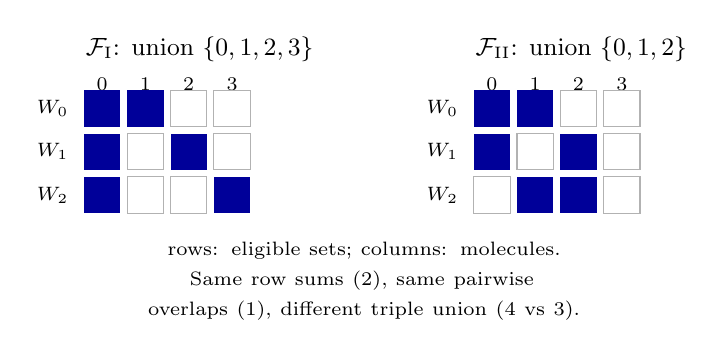
\begin{tikzpicture}[x=0.55cm,y=0.55cm,font=\small]
\foreach \fam/\xo/\name/\rows in {I/0/{$\cF_{\mathrm I}$: union $\{0,1,2,3\}$}/{{1,1,0,0},{1,0,1,0},{1,0,0,1}}, II/9/{$\cF_{\mathrm{II}}$: union $\{0,1,2\}$}/{{1,1,0,0},{1,0,1,0},{0,1,1,0}}}{
  \node[anchor=south west] at (\xo-0.1,3.35) {\name};
  \foreach \c in {0,1,2,3}{\node at (\xo+\c+0.5,3.05) {\scriptsize\c};}
  \foreach \r [count=\ri from 0] in \rows {
    \foreach \v [count=\c from 0] in \r {
      \pgfmathparse{\v}
      \ifnum\pgfmathresult=1
        \fill[blue!60!black] (\xo+\c+0.08,2.08-\ri) rectangle (\xo+\c+0.92,2.92-\ri);
      \else
        \draw[gray!60] (\xo+\c+0.08,2.08-\ri) rectangle (\xo+\c+0.92,2.92-\ri);
      \fi
    }
    \node[anchor=east] at (\xo-0.05,2.5-\ri) {\scriptsize $W_{\ri}$};
  }
}
\node[anchor=north,align=center,text width=5.6cm] at (6.5,-0.35) {\scriptsize rows: eligible sets; columns: molecules.\\ Same row sums (2), same pairwise overlaps (1), different triple union (4 vs 3).};
\end{tikzpicture}
\caption{Incidence matrices of the two three-set families of Theorem~\ref{thm:pairwise}. All statistics of order at most two agree; the third-order union term $q^{|W_0\cup W_1\cup W_2|}$ differs.}
\label{fig:pairwise}
\end{figure}

\begin{corollary}\label{cor:pairwise}
Any formula for the activation probability of a family of cores that depends only on the eligible-set sizes and pairwise intersection sizes on each channel assigns the same value to a channel carrying $\cF_{\mathrm I}$ and to one carrying $\cF_{\mathrm{II}}$, and is therefore wrong for at least one of them whenever $0<q<1$.
\end{corollary}

The corollary does not say that pair-corrected formulas are useless: they are second-order Bonferroni-type truncations of Theorem~\ref{thm:global}~\cite{galambos1996bonferroni}, and their error is governed by the third and higher union terms. It says that ``pair-corrected'' is not synonymous with ``exact''.

\section{Recovery of the non-overlap formula}\label{sec:nonoverlap}

The finite-core theory of~\cite{varanasi2026emergence} combines one-core probabilities $\pi_k$ as if the cores were independent, $\Pr(\text{some core})=1-\prod_k(1-\pi_k)$. We identify the exact hypothesis under which this is an identity rather than an approximation: the cores must occupy pairwise disjoint blocks of catalysis coordinates.

\begin{definition}[Dedicated coordinates]
Given eligible sets $W_k\subseteq M$ ($k\in\cK$) and a finite set $\Phi$ of fibre labels, the dedicated channel set is $\cK\times\Phi$ and the requirement of core $k$ on channel $(k',\varphi)$ is $W_k$ if $k'=k$ and $\varnothing$ otherwise \textup{(\lean{dedicatedRequirements})}.
\end{definition}

\begin{theorem}[Non-overlap specialisation]\label{thm:nonoverlap}
With dedicated coordinates, all $W_k\neq\varnothing$, and $m=|\Phi|$:
\begin{enumerate}[label=\textup{(\roman*)}]
\item for every $\cA\subseteq\cK$, $\Pr_p\bigl(\bigcap_{k\in\cA}E_k\bigr)=\prod_{k\in\cA}\Pr_p(E_k)$;
\item $\Pr_p(E_k)=\bigl[1-(1-p)^{|W_k|}\bigr]^{m}$;
\item $\displaystyle\Pr_p(E_\cK)=1-\prod_{k\in\cK}\Bigl(1-\bigl[1-(1-p)^{|W_k|}\bigr]^{m}\Bigr)$.
\end{enumerate}
\leanrefs{\lean{dedicated\_intersections\_factorize}, \lean{jointBernoulliHitProbability\_dedicated}, \lean{rafBernoulliProbability\_dedicated\_nonoverlap}}
\end{theorem}

\begin{proof}
On the dedicated channel $(k',\varphi)$ the requirement family of $\cA$ is $\{W_{k'}\}$ if $k'\in\cA$ and empty otherwise, so by the two elementary cases of Section~\ref{sec:local} the joint probability is $\prod_{k\in\cA}(1-(1-p)^{|W_k|})^{m}$, which is (i) and (ii). Substituting a factorising family into Theorem~\ref{thm:global}(i) and using the identity $\sum_{\varnothing\ne\cA}(-1)^{|\cA|+1}\prod_{k\in\cA}\pi_k=1-\prod_k(1-\pi_k)$ (\lean{independentCoreUnionExpansion}) gives (iii).
\end{proof}

Theorem~\ref{thm:nonoverlap} locates the approximation of the finite-core theory precisely. The one-core marginals $[1-(1-p)^{w}]^{m}$ are correct, and are exactly the singleton case of Theorem~\ref{thm:local}. What the non-overlap assumption changes is the geometry of intersections: shared molecules on shared channels are replaced by private copies. The general formula, Theorem~\ref{thm:global}, keeps the marginals and replaces the product of marginals by the union trace of Remark~\ref{rem:statistic}. Comparing two models with the same marginals and different traces isolates the effect of network geometry from the effect of the catalysis level.

\section{The finite food gateway}\label{sec:gateway}

The results so far are exact at every finite $n$. The asymptotic content of the paper comes from a structural feature of the fixed-food model: while $|X_n|$ and $|J_n|$ grow exponentially, the number of channels through which a RAF can be entered from food does not grow at all.

\begin{figure}[t]
\centering
\resizebox{\textwidth}{!}{%
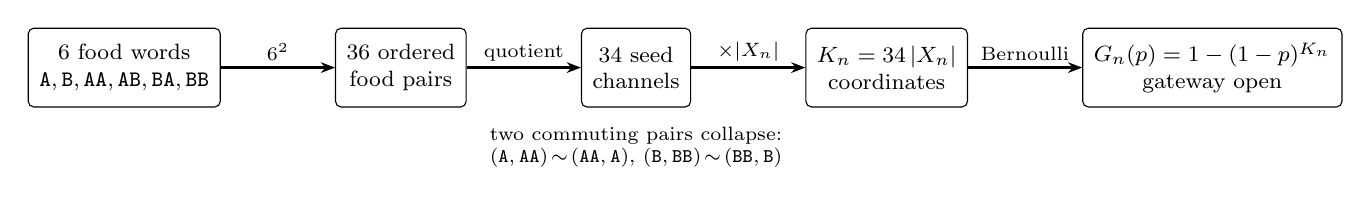
\begin{tikzpicture}[font=\footnotesize,node distance=0.5cm and 1.45cm,
  box/.style={draw,rounded corners=2pt,align=center,inner sep=4pt,minimum height=1.0cm},
  lab/.style={font=\scriptsize,align=center,inner sep=1pt},
  arr/.style={-{Stealth[length=1.8mm]},thick}]
\node[box] (food) {6 food words\\ $\word{A},\word{B},\word{AA},\word{AB},\word{BA},\word{BB}$};
\node[box,right=of food] (pairs) {36 ordered\\ food pairs};
\node[box,right=of pairs] (quot) {34 seed\\ channels};
\node[box,right=of quot] (coord) {$K_n=34\,|X_n|$\\ coordinates};
\node[box,right=of coord] (prob) {$G_n(p)=1-(1-p)^{K_n}$\\ gateway open};
\draw[arr] (food) -- (pairs) node[midway,above=1pt,lab] {$6^2$};
\draw[arr] (pairs) -- (quot) node[midway,above=1pt,lab] {quotient};
\draw[arr] (quot) -- (coord) node[midway,above=1pt,lab] {$\times|X_n|$};
\draw[arr] (coord) -- (prob) node[midway,above=1pt,lab] {Bernoulli};
\node[below=0.2cm of quot,lab] {two commuting pairs collapse:\\ $(\word{A},\word{AA})\!\sim\!(\word{AA},\word{A})$, $(\word{B},\word{BB})\!\sim\!(\word{BB},\word{B})$};
\end{tikzpicture}}
\caption{The repository gateway at food horizon $2$ and $n\ge4$. Exactly two of the $36$ ordered food pairs are identified by the commuting-factor quotient, leaving $34$ seed channels; each carries $|X_n|$ independent catalysis coordinates.}
\label{fig:gateway}
\end{figure}

\subsection{Exactly 34 seed channels}

Products of two food words have length at most $4$. Once $n\ge4$ every ordered pair of food words is an admissible channel, and the seed channels are exactly the (quotiented) food pairs: a channel with $\rhs\subseteq F$ has a product of length at most $2$, hence factors of length $1$, and is a food pair as well. Among the $36$ ordered food pairs the commuting distinct pairs are $\{\word{A},\word{AA}\}$ and $\{\word{B},\word{BB}\}$, each collapsed once.

\begin{theorem}[Exact seed count]\label{thm:34}
For every $n\ge4$, $|\seed_2(n)|=34$.
\leanrefs{\lean{repositorySeedChannels\_card\_eq\_34}}
\end{theorem}

\begin{proof}
Let $\Gamma$ be the intrinsic gateway type: ordered pairs $(u,v)$ of words of length at most $2$ with $uv\neq vu$ or $u\preceq v$ (\lean{RepositoryGateway 2}). Kernel evaluation gives $|\Gamma|=34$ (\lean{card\_repository\_gateway\_binary\_t2}). \emph{Upper bound}, valid for all $n$: a seed channel has both factors in $F$ (if $\lhs\subseteq F$ this is immediate; if $\rhs\subseteq F$ the product has length at most $2$, so each factor has length $1$). Truncating the two factors to words of length at most $2$ preserves length and code, hence preserves the canonicity condition, and gives an injection $\seed_2(n)\to\Gamma$ (\lean{repositorySeedChannels\_card\_le\_34}). \emph{Lower bound}, for $n\ge4$: embedding a pair in $\Gamma$ into $X_n\times X_n$ preserves lengths and codes; the product fits because $|u|+|v|\le4\le n$; the canonicity condition transfers verbatim; and $\lhs=\{u,v\}\subseteq F$, so the image is a seed channel. This map is injective (\lean{repositoryGatewayToSeedChannel\_injective}).
\end{proof}

The theorem is a stabilisation statement across all $n\ge4$, not a computation at one $n$. It also explains the difference between the two conventions: in the split-position catalogue the same argument yields $36$ seed reactions, the count used in~\cite{criticalwindow2026}.

\subsection{Every RAF crosses the gateway}

\begin{theorem}[Seed necessity]\label{thm:necessity}
Let $\cQ$ be any reversible system, $C$ a catalysis relation and $S$ a set of channels with $\mathrm{IsRevRAF}(\cQ,C,S)$. Then there exist a seed channel $r$ and a molecule $x$ with $C(x,r)$; moreover $r\in S$ and $x$ is reachable in the closure of $S$.
\leanrefs{\lean{rev\_raf\_implies\_seedOpen}, \lean{repository\_raf\_has\_catalyzed\_gateway}}
\end{theorem}

\begin{proof}
If no channel of $S$ were a seed, no side of any channel of $S$ would be contained in $\cl^0_S=F$, so $\cl^1_S=F$, and by induction $\cl^k_S=F$ for all $k$ (\lean{revClosureAt\_eq\_food\_of\_no\_seed}). Take any $r\in S$; food generation gives $k$ with $\lhs(r)\subseteq\cl^k_S=F$, so $r$ is a seed after all. Reflexive autocatalysis supplies its catalyst.
\end{proof}

\subsection{The probability cap}

Let $\Gamma$ and $K_n=|X_n|\cdot|\Gamma|=34(2^{n+1}-2)$ be as above (\lean{repositoryGatewayCoordinateCount}), and define the gateway-open probability
\[
G_n(p)=1-(1-p)^{K_n}\qquad(\lean{repositoryGatewayOpenProbability}).
\]
For $n\ge4$ this is exactly the Bernoulli probability that some seed channel is catalysed by some molecule; for smaller $n$ it is an upper bound for that probability.

\begin{theorem}[Gateway cap]\label{thm:cap}
For every $n\ge1$ and $p\in[0,1]$, with $\cK=\cK_{n,2}$,
\[
0\ \le\ \Pr_p\bigl(\RAF_n\bigr)\ \le\ \Pr_p(\text{some seed channel catalysed})\ \le\ G_n(p)\ \le\ K_np .
\]

\leanrefs{\lean{jointFibreBernoulliWeight\_nonneg}, \lean{repositoryRAFBernoulliProbability\_le\_seedOpen}, \lean{repositoryRAFBernoulliProbability\_le\_gateway}, \lean{repositoryGatewayOpenProbability\_le}}
\end{theorem}

\begin{proof}
Model the seed-open event as a catalogue in the sense of Section~\ref{sec:semantic}: one core per seed channel $r$, with requirement $W_{r,j}=X_n$ if $j=r$ and $\varnothing$ otherwise (\lean{repositorySeedRequirements}). Its cores are coordinate-disjoint, so Theorem~\ref{thm:nonoverlap} gives the exact probability $1-(1-p)^{|X_n|\,|\seed_2(n)|}$ (\lean{repositorySeedOpenProbability\_exact}). By Theorems~\ref{thm:semantic} and~\ref{thm:necessity}, every configuration in the RAF event lies in the seed-open event (\lean{repositoryRAFFibreConfigurations\_subset\_seedOpenConfigurations}), and Bernoulli weights are nonnegative, which gives the first two inequalities. The third is $|\seed_2(n)|\le34$ from Theorem~\ref{thm:34}, and the last is the union bound $1-(1-p)^K\le Kp$.
\end{proof}

We stress that the containment in Theorem~\ref{thm:cap} is proved for the actual RAF event, using the exhaustive catalogue and Theorem~\ref{thm:semantic}. An earlier version of the development stated the asymptotic results for an arbitrary probability sequence dominated by $G_n$; this was replaced because such a statement leaves the essential step, that the RAF event is inside the seed-open event, to the reader.

\section{Asymptotic consequences}\label{sec:asymptotics}

Throughout this section the food horizon is $t=2$, $p_n=f_n/|J_n|$, and $\Pr(\RAF_n)$ denotes the Bernoulli probability of the actual RAF event (\lean{repositoryRAFBernoulliProbability}).

\subsection{Sublinear catalysis}

\begin{proposition}[Quantitative cap]\label{prop:272}
For $n\ge3$ and $0\le f_n\le|J_n|$, \; $G_n(p_n)\le 272\,f_n/n$.
\leanrefs{\lean{repositoryGatewayOpenProbability\_le\_sublinearScale}}
\end{proposition}

\begin{proof}
By Theorem~\ref{thm:cap}, $G_n(p_n)\le K_np_n=34\,f_n\,|X_n|/|J_n|$. Now $|X_n|\le 2\cdot2^n$ and, by~\eqref{eq:lower}, $|J_n|\ge\lfloor(n-1)/2\rfloor2^n\ge(n/4)2^n$ for $n\ge3$. Hence $|X_n|/|J_n|\le8/n$ and $G_n(p_n)\le 272f_n/n$.
\end{proof}

The constant $272=34\cdot8$ is deliberately coarse. Proposition~\ref{prop:count} would replace $8$ by $2+o(1)$, but the formal development uses only~\eqref{eq:lower}, which is all that is needed for the scale separation.

\begin{theorem}[Sublinear catalysis forces RAF probability to vanish]\label{thm:sublinear}
Let $f:\Nat\to\Real$ satisfy $0\le f_n\le|J_n|$ for all $n$ and $f_n/n\to0$. Then $\Pr(\RAF_n)\to0$. In particular this holds for every constant $f$.
\leanrefs{\lean{sublinear\_catalysis\_forces\_actual\_repository\_raf\_vanishing}}
\end{theorem}

\begin{proof}
For $n\ge3$, Theorem~\ref{thm:cap} and Proposition~\ref{prop:272} give $0\le\Pr(\RAF_n)\le272f_n/n\to0$.
\end{proof}

\subsection{Linear catalysis}

Every fixed $f$ is sublinear, so the first scale not excluded by Theorem~\ref{thm:sublinear} is $f_n=\lambda n$. On that scale the expected number of open gateway coordinates stays bounded.

\begin{lemma}\label{lem:linear}
For $\lambda\ge0$ and $n\ge3$, $p_n K_n\le272\lambda$ when $f_n=\lambda n$; and $K_n\to\infty$.
\leanrefs{\lean{repository\_linear\_rate\_mul\_gatewayCoordinateCount\_le}, \lean{repositoryGatewayCoordinateCount\_tendsto}}
\end{lemma}

\begin{proof}
$p_nK_n=34\lambda n|X_n|/|J_n|\le 34\lambda n\cdot 8/n$ by the estimates in the proof of Proposition~\ref{prop:272}; and $K_n\ge 2^n$.
\end{proof}

\begin{theorem}[Finite linear catalysis cannot force RAF probability to one]\label{thm:linear}
For every real $\lambda>0$, the sequence $\Pr(\RAF_n)$ at $f_n=\lambda n$ does not converge to $1$.
\leanrefs{\lean{linear\_catalysis\_actual\_repository\_raf\_not\_tendsto\_one}}
\end{theorem}

\begin{proof}
Put $C=272\lambda$. By Lemma~\ref{lem:linear}, eventually $C\le K_n$ and $p_n\le C/K_n$. Since $(1-C/K_n)^{K_n}\to\ee^{-C}$, there is $\delta>0$ with $(1-p_n)^{K_n}\ge(1-C/K_n)^{K_n}\ge\delta$ for all large $n$ (\lean{bernoulli\_absent\_eventually\_pos}). By Theorem~\ref{thm:cap}, $\Pr(\RAF_n)\le1-(1-p_n)^{K_n}\le1-\delta$ eventually, which is incompatible with convergence to $1$.
\end{proof}

The theorem says that the boundary keeps a non-vanishing influence at every finite linear rate: with positive probability bounded away from zero, none of the $34$ entry channels is catalysed and no RAF can exist. It does not determine $\lim\Pr(\RAF_n)$, nor assert that the limit exists.

\subsection{The exact boundary--bulk factorisation}

\begin{proposition}[Gateway-conditioned bulk factor]\label{prop:bulk}
For every $n$ and $p$ with $G_n(p)\neq0$ define $B_n(p)=\Pr_p(\RAF_n)/G_n(p)$. Then $\Pr_p(\RAF_n)=G_n(p)\,B_n(p)$.
\leanrefs{\lean{repositoryRAFBernoulliProbability\_gateway\_factorization}}
\end{proposition}

The identity is algebraic and asserts no independence. By Theorem~\ref{thm:cap}, $0\le B_n(p)\le1$ for $p\in(0,1]$, and for $n\ge4$, where $G_n(p)$ is exactly the seed-open probability, $B_n(p)$ is the conditional probability of a RAF given that some seed channel is catalysed. Its purpose is to name the object that remains to be understood: all unresolved large-$n$ behaviour on the linear scale lives in $B_n(\lambda n/|J_n|)$.

\subsection{The sharp gateway constant}

\begin{corollary}[Sharp gateway limit; not formalised]\label{cor:sharp}
For every $\lambda\ge0$, $\;G_n\bigl(\lambda n/|J_n|\bigr)\to1-\ee^{-34\lambda}$.
\end{corollary}

\begin{proof}
By Proposition~\ref{prop:count}, $|J_n|=(n-2)2^{n+1}(1+o(1))$, so $p_nK_n=34\lambda n(2^{n+1}-2)/|J_n|\to34\lambda$, while $p_n\to0$. Hence $K_n\log(1-p_n)=-p_nK_n(1+O(p_n))\to-34\lambda$ and $(1-p_n)^{K_n}\to\ee^{-34\lambda}$.
\end{proof}

Figure~\ref{fig:curves}(a) shows the exact finite curves $G_n(\lambda n/|J_n|)$ computed from the closed form of Proposition~\ref{prop:count}; at $\lambda=0.03$ the value moves from $0.7848$ at $n=6$ to $0.6511$ at $n=64$ against the limit $1-\ee^{-1.02}\approx0.6394$. The convergence is slow, of order $1/n$, because $n|X_n|/|J_n|=(n/(n-2))(1+o(1))$. Together with Proposition~\ref{prop:bulk} the corollary gives the exact asymptotic decomposition on the linear scale,
\[
\Pr(\RAF_n)=\bigl(1-\ee^{-34\lambda}+o(1)\bigr)\,B_n\bigl(\lambda n/|J_n|\bigr),
\]
and reduces the emergence problem at that scale to the bulk factor. The corollary is not needed for any of Theorems~\ref{thm:sublinear} and~\ref{thm:linear}, which rest only on~\eqref{eq:lower}.

\begin{figure}[t]
\centering
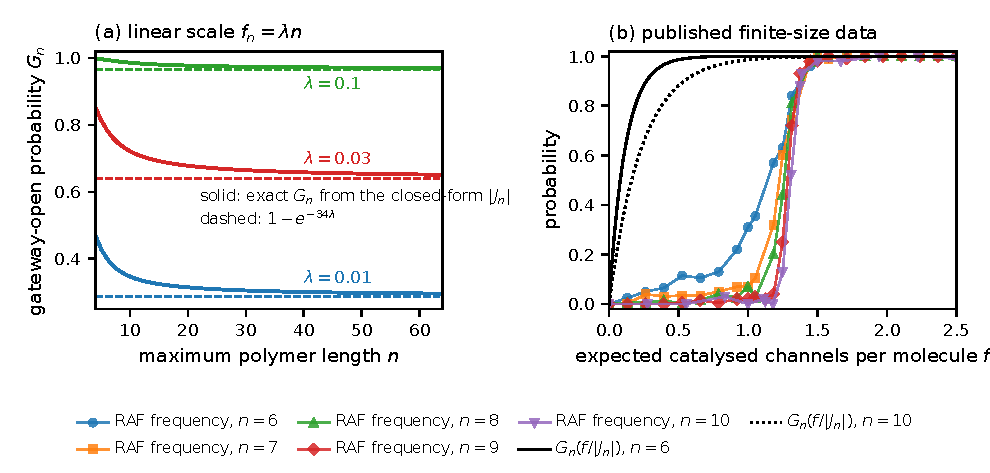
\includegraphics[width=\textwidth]{figures/gateway_curves.pdf}
\caption{(a) Exact gateway-open probability $G_n(\lambda n/|J_n|)$ for $\lambda\in\{0.01,0.03,0.1\}$ with $|J_n|$ from Proposition~\ref{prop:count}, against the limits $1-\ee^{-34\lambda}$ of Corollary~\ref{cor:sharp}. (b) The $111$ RAF frequencies published in~\cite{varanasi2026repository} for $n=6,\dots,10$ as a function of $f$, with the exact gateway curves $G_n(f/|J_n|)$ for $n=6$ and $n=10$. In the finite transition window the gateway is almost surely open; the finite curve is not shaped by it.}
\label{fig:curves}
\end{figure}

\section{Numerical diagnostics}\label{sec:numerics}

Numerical work was used to discriminate conventions and to motivate statements, never as evidence for a theorem. Three small exact computations were decisive.

\paragraph{Reaction census.}
A semantic re-implementation of the repository generator (which records displayed reactant and product lists and suppresses duplicates) was compared with Proposition~\ref{prop:count} for $n=2,\dots,8$ (Table~\ref{tab:census}). The counts agree, every directed record is followed by its exact reverse, and the seed count stabilises at $34$ from $n=4$. The mismatch with the split-position catalogue at $n=3$ ($18$ versus $20$) was the observation that forced the reconstruction of the quotient before any probability theorem was attempted.

\begin{table}[t]
\centering\small
\caption{Exact census of the repository generator (binary alphabet, food horizon $2$). ``Split'' is the split-position count $(n-2)2^{n+1}+4$; ``$C(n)$'' is the commuting-pair correction of Proposition~\ref{prop:count}.}
\label{tab:census}
\begin{tabular}{@{}rrrrrrr@{}}
\toprule
$n$ & $|X_n|$ & directed reactions & $|J_n|$ & split & $C(n)$ & seed channels\\
\midrule
2 & 6 & 8 & 4 & 4 & 0 & 4\\
3 & 14 & 36 & 18 & 20 & 2 & 18\\
4 & 30 & 128 & 64 & 68 & 4 & 34\\
5 & 62 & 376 & 188 & 196 & 8 & 34\\
6 & 126 & 1004 & 502 & 516 & 14 & 34\\
7 & 254 & 2528 & 1264 & 1284 & 20 & 34\\
8 & 510 & 6096 & 3048 & 3076 & 28 & 34\\
\bottomrule
\end{tabular}
\end{table}

\paragraph{Single-catalyst witnesses.}
The repository file \texttt{single\_solutions.json} lists $96$ single-catalyst RAF witnesses at $n=6$. Each is a pair of adjacent directed indices, that is one reversible channel, together with one catalyst molecule lying in the closure of that channel. The $96$ witnesses are supported on exactly $34$ distinct channels, the seed channels of Theorem~\ref{thm:34}. This illustrates the distinction, built into Section~\ref{sec:semantic}, between a reaction-support core and a catalyst-labelled witness of it: treating the $96$ objects as $96$ cores in the outer inclusion--exclusion would count the same event many times.

\paragraph{Gateway versus the finite transition.}
Figure~\ref{fig:curves}(b) overlays the $111$ published RAF frequencies with the exact gateway curve. At the observed transition the gateway is already almost surely open: at $n=6$ and $f\approx1.316$ the RAF frequency is $0.84$ while $G_6=0.99999$; at $n=10$ and $f=1.31$ the $25$-run estimate is $0.52$ while $G_{10}=0.9962$. The gateway therefore does not shape the finite-size curve. Its role is asymptotic: at fixed $f$ the same curve cannot persist, because $G_n(f/|J_n|)=O(f/n)$.

\paragraph{Performance.}
No enumeration of catalysis configurations was performed anywhere on the proof path. The pairwise-insufficiency fixture is evaluated exhaustively inside Lean on a four-element set; the channel and gateway counts at $n=3$ and horizon $2$ are kernel evaluations on types of size at most $14^2$.

\section{Formal verification}\label{sec:verification}

The development is organised in four layers under \lean{proofs/OverlapCorrectedRAF/}: \lean{Source} (the repository quotient, its reversible system, the semantic catalogue, the gateway dock, and the exact seed count), \lean{Core} (finite core events and one-core probabilities), \lean{Overlap} (local hit polynomials, semantic counting, the finite partition, the pairwise counterexample, and the non-overlap specialisation), and \lean{Asymptotic} (gateway probability, sublinear and linear catalysis, and the bulk factorisation). The terminal theorem, \lean{OverlapCorrectedRAF.correctedEmergenceResolution}, takes as hypotheses natural numbers $n,t,Q$, a real $f$, a catalysis relation $C$ and a channel set $S$ with $\mathrm{IsRevRAF}(\cQ_{n,t},C,S)$, and a sequence $f:\Nat\to\Real$ with $0\le f_m\le|J_m|$ for all $m$ and $f_m/m\to0$. It concludes the conjunction of \lean{HasExactRepositoryRAFLaw}$\,n\,t\,Q$, of the existence of a seed channel $r$ and a molecule $x$ with $C(x,r)$, and of $\Pr(\RAF_m)\to0$, which packages Corollary~\ref{cor:repolaw}, Theorem~\ref{thm:necessity} and Theorem~\ref{thm:sublinear}. The post-proof modules add Theorems~\ref{thm:34} and~\ref{thm:linear} and Proposition~\ref{prop:bulk}. All modules compile under Lean~4.30.0 against a frozen Mathlib with \lean{-DwarningAsError=true}, exit code zero, and no \lean{sorry}. Table~\ref{tab:receipts} lists the SHA-256 hashes (first 16 hexadecimal digits) of the sources and of the compiled artefacts. The reproduction command from the repository root is
\begin{center}\small
\lean{py scripts/verify\_proof.py proofs/OverlapCorrectedRAF/CorrectedEmergenceResolution.lean}
\end{center}

\begin{table}[t]
\centering\small
\caption{Verification receipts. Hashes are SHA-256, truncated to 16 hexadecimal digits; the full values are recorded in the repository handoff.}
\label{tab:receipts}
\begin{tabular}{@{}lll@{}}
\toprule
Module & source & artefact\\
\midrule
\lean{Overlap/FinitePartition.lean} & \lean{a3c94dced502d88c} & \lean{21113c5713af0117}\\
\lean{Overlap/SemanticCounting.lean} & \lean{d091c8ceca281272} & \lean{0105b89a98eb287a}\\
\lean{Overlap/TriplePairwiseFailure.lean} & \lean{9622c13de8d246fb} & \lean{40fd1d100a89eb15}\\
\lean{Overlap/Nonoverlap.lean} & \lean{3bd660e9ccd9d688} & \lean{42b28a1d9f013ecb}\\
\lean{Source/RepositorySemanticCounting.lean} & \lean{4929e5fe8f5d8318} & \lean{83d27e083680a59e}\\
\lean{Source/ActualGatewayDock.lean} & \lean{7c22a10632f2201a} & \lean{827f33ad5ccff87a}\\
\lean{Source/ExactSeedChannels.lean} & \lean{1a4abdf9ea110b2a} & \lean{bf93795fce3b7271}\\
\lean{Asymptotic/SublinearCatalysis.lean} & \lean{ec241b57f7766fee} & \lean{dd94a0946dfaf8ca}\\
\lean{Asymptotic/LinearCatalysis.lean} & \lean{23d37db67fb5ebff} & \lean{66e0cd9d11de5195}\\
\lean{Asymptotic/GatewayConditionedBulk.lean} & \lean{aac959e41cda9510} & \lean{d07f7b82eed0f38a}\\
\lean{CorrectedEmergenceResolution.lean} & \lean{7aa9018c0c15aadb} & \lean{27ec5bbe0e46db17}\\
\bottomrule
\end{tabular}
\end{table}

Two remarks on what the formalisation forced. First, the exact formulas of Sections~\ref{sec:local} and~\ref{sec:global} were initially \emph{definitions}; they became theorems only when each polynomial was proved equal to the generating polynomial of an explicit finite set of configurations (\lean{fibreHitConfigurations}, \lean{jointFibreHitConfigurations}, \lean{catalogueFibreHitConfigurations}) and those sets were identified with the RAF event. Second, the fixed-$Q$ probability has codomain $\Real$, with the integer numerator and binomial denominator cast before division; a natural-number quotient would not define a probability. Both points are invisible in informal presentations and both were caught by the type checker.

\section{Discussion}\label{sec:discussion}

\subsection*{What is and is not claimed}

The paper proves an exact finite law, identifies its sufficient statistic, shows that pairwise data are not sufficient, recovers the independent-core formula under coordinate disjointness, establishes the exact $34$-channel gateway, and derives the sublinear vanishing and finite-linear obstruction theorems for the actual RAF event of the repository model. It also proves by hand, outside Lean, the closed-form channel count and the sharp gateway limit.

It does not claim a positive RAF limit at $f_n=\lambda n$, a transition width, a Poisson law for the number of cores, or a decay rate for connected overlap clusters. It does not claim that the gateway explains the shape of the finite transition; Section~\ref{sec:numerics} shows that it does not. It does not claim computational efficiency for Theorem~\ref{thm:global}. It does not identify the repository quotient with the split-position model, nor the Bernoulli with the fixed-$Q$ ensemble, nor the $96$ catalyst witnesses with $96$ cores. The homogeneous ensembles are essential to Remark~\ref{rem:statistic}: for molecule-dependent or correlated catalysis distributions~\cite{hordijk2016variable} the local law would need the full set-valued trace $\{\bigcup\cT\}$ rather than its cardinalities, and the fixed-$Q$ ensemble would no longer be determined by $Q$ alone.

\subsection*{Interpretation}

Three structural facts, rather than one, were hidden in the phrase ``overlapping cores''. The first is that dependence between cores is a third- and higher-order phenomenon on each channel, so the correct state variable is a union trace. The second is that the reaction identity of the source is a quotient of the textbook catalogue, so an exact theorem must be proved in the quotient. The third is that a fixed food set is a boundary of bounded size in a system whose bulk grows exponentially; the exponentially many catalyst molecules do not compensate, because the per-coordinate probability shrinks at exactly the compensating rate $f/|J_n|$. The finite-size transition near $f\approx1.3$ is real, and the finite-core theory describes it; what the gateway forbids is the extrapolation of a constant-$f$ transition to $n\to\infty$.

\subsection*{Open problems}

\begin{enumerate}[label=\textup{(\arabic*)}]
\item \emph{The bulk factor.} Determine the behaviour of $B_n(\lambda n/|J_n|)$ as $n\to\infty$. For the split-position catalogue the companion manuscript~\cite{criticalwindow2026} proves that the RAF probability itself converges to $\Theta(\lambda)=S(1-\ee^{-\lambda})$, a nondecreasing continuous function with $0<\Theta<1$ on $(0,\infty)$, so that no finite $\lambda$ separates limit $0$ from limit $1$. Transferring that analysis to the repository quotient, where Corollary~\ref{cor:sharp} fixes the gateway factor at $1-\ee^{-34\lambda}$, would determine $\lim B_n$; it is open whether the two conventions have the same bulk limit.
\item \emph{Compression of the trace.} Quotient the union trace to a coverage polynomial whose coefficients group equal union cardinalities, and determine when this smaller statistic is exact for homogeneous catalysis.
\item \emph{Support cores versus witnesses.} Formalise the resummation from catalyst-labelled minimal witnesses to reaction-support cores that explains the $96\to34$ collapse in general.
\item \emph{Cluster factorisation.} Cores with disjoint coordinate sets are independent under Bernoulli catalysis; factor the no-RAF probability over connected components of the overlap graph and use it as the basis for cluster expansions and bounded-width dynamic programmes.
\item \emph{Universality of finite gateways.} Abstract the argument of Section~\ref{sec:gateway} to random catalytic systems with a uniformly bounded mandatory boundary set, per-coordinate probability $f_n/|J_n|$ and molecule-to-channel ratio of order $1/n$, and formalise Proposition~\ref{prop:count} and Corollary~\ref{cor:sharp}.
\end{enumerate}

\subsection*{Data and code availability}

The Lean sources, the exact census scripts, the audit of the single-catalyst fixture, the $111$ published RAF frequencies used in Figure~\ref{fig:curves}, and the script that generates that figure are available in the public repository \url{https://github.com/mmislan/Erdos} under \lean{proofs/OverlapCorrectedRAF/}, \lean{problem\_workspaces/RAF\_overlap\_corrected\_Kauffman\_emergence/} and \lean{key\_results/RAFs/}.

\bibliographystyle{plain}
\bibliography{refs}

\end{document}
